\documentclass[12pt,a4paper]{article}

\usepackage{tikz-feynman}
\usepackage{amsmath}

\begin{document}
qweqwe
\begin{figure}
    \centering
    \feynmandiagram [layered layout, horizontal=a to b] {
        a [particle=\(\mu^{-}\)] -- [fermion] b 
        -- [fermion, edge label=\(\nu\), half left, looseness=1.7] c
        -- [boson, edge label=\(W^-\), half left, looseness=1.8] b,
        c -- [fermion, particle=\(\nu_\mu\)] d,
        %b -- [boson, edge label'=\(W^{-}\)] c,
        %c -- [anti fermion] f2 [particle=\(\overline \nu_{e}\)],
        %c -- [fermion] f3 [particle=\(e^{-}\)],
    };
        \caption{
            Feynman diagram for $\mu \rightarrow e + \gamma$ allowed by
            flavour oscillation of a virtual neutrino.
        }
    \label{fig:mu_e_nu_osc}
\end{figure}

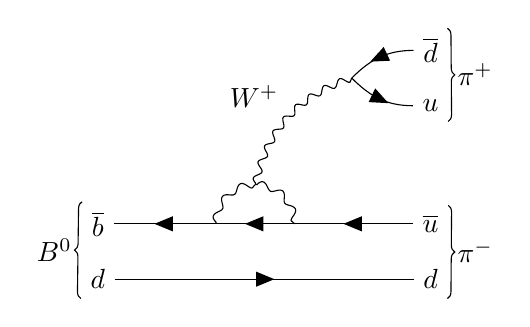
\begin{tikzpicture}
\begin{feynman}
    \vertex (a1) {\(\overline b\)};
    \vertex[right=1.5cm of a1] (a2);
    \vertex[right=1cm of a2] (a3);
    \vertex[right=1.5cm of a3] (a4) {\(\overline u\)};
    \vertex[below=2em of a1] (b1) {\(d\)};
    \vertex[below=2em of a4] (b2) {\(d\)};
    %% See section 13.5 of PGF/TikZ manual
    \vertex at ($(a2)!0.5!(a3)!0.5cm!90:(a3)$) (d);
    %% Equivalent way to obtain (d):
    % \vertex at ($(b2)!0.5!(b3) + (0, -0.5cm)$) (d);
    \vertex[above=of a4] (c1) {\(u\)};
    \vertex[above=2em of c1] (c3) {\(\overline d\)};
    \vertex at ($(c1)!0.5!(c3) - (1cm, 0)$) (c2);
    \diagram* {
    (a4) -- [fermion] (a3) -- [fermion] (a2) -- [fermion] (a1),
    (b1) -- [fermion] (b2),
    (c3) -- [fermion, out=180, in=45] (c2) -- [fermion, out=-45, in=180] (c1),
    (a2) -- [boson, quarter left] (d) -- [boson, quarter left] (a3),
    (d) -- [boson, bend left, edge label=\(W^{+}\)] (c2),
    };
    \draw [decoration={brace}, decorate] (b1.south west) -- (a1.north west)
    node [pos=0.5, left] {\(B^{0}\)};
    \draw [decoration={brace}, decorate] (c3.north east) -- (c1.south east)
    node [pos=0.5, right] {\(\pi^{+}\)};
    \draw [decoration={brace}, decorate] (a4.north east) -- (b2.south east)
    node [pos=0.5, right] {\(\pi^{-}\)};
\end{feynman}
\end{tikzpicture}

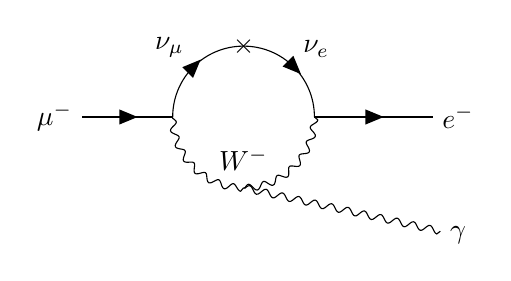
\begin{tikzpicture}
\begin{feynman}
\vertex (a) {\(\mu^{-}\)};
\vertex [right=1.5cm of a] (b);
\vertex [right=1.8cm of b] (c);
\vertex [right=1.5cm of c] (d) {\(e^-\)};

\vertex at ($(b)!0.5!(c) + (0, 0.9cm)$) (n);
\vertex at ($(b)!0.5!(c) + (0, -0.9cm)$) (w);
\vertex [above=0.1cm of w] (wn) {\(W^-\)};
\vertex [below=1.5cm of d] (g) {\(\gamma\)};

\diagram* {
(a) -- [fermion] (b)
-- [fermion, quarter left, edge label=\(\nu_\mu\)] (n)
-- [fermion, quarter left, edge label=\(\nu_e\)] (c),
(b) -- [boson, quarter right] (w)
-- [boson, quarter right] (c),
(c) -- [fermion] (d),
(w) -- [boson] (g),
};

\draw (n) -- (n) node {\(\times\)};

\end{feynman}
\end{tikzpicture}



\begin{figure}
    \centering
    \feynmandiagram [medium, vertical=b to d] {
        a [particle=\(\mu^{-}\)] -- [fermion] b [blob]
        -- [fermion] c [particle=\(e\)],
        b -- [boson] d [particle=\(\gamma\)],
        %b -- [boson, edge label'=\(W^{-}\)] c,
        %c -- [anti fermion] f2 [particle=\(\overline \nu_{e}\)],
        %c -- [fermion] f3 [particle=\(e^{-}\)],
    };
    \hspace{3cm}
    \feynmandiagram [medium, horizontal=a to c] {
        a [particle=\(\mu^{-}\)] -- [fermion] b [blob]
        -- [fermion] c [particle=\(e\)],
        e  [particle=\(q\)] -- [fermion] b,
        b -- [fermion] d [particle=\(q\)],
        %b -- [boson, edge label'=\(W^{-}\)] c,
        %c -- [anti fermion] f2 [particle=\(\overline \nu_{e}\)],
        %c -- [fermion] f3 [particle=\(e^{-}\)],
    };
    \caption{
        wewwee
    }
    \label{fig:mu_e_nu_osc}
\end{figure}

\begin{align}\label{eq:Leff}
    \mathcal{L^\text{eff}_\mathrm{CLFV}} 
    = \ 
    &\frac{1}{\kappa+1}\,\frac{m_\mu}{\Lambda^2}\,
    \overline{\mu}_R \sigma_{\mu\nu} e_L F^{\mu\nu} + \text{h.c.}
    \nonumber\\[1em]
    + \  &\frac{\kappa}{\kappa+1} \frac{1}{\Lambda^2}\,
    \overline{\mu}_L \gamma_\mu e_L \,
    ( 
        \overline{u}_L \gamma^\mu u_L + \overline{d}_L \gamma^\mu d_L
    ) + \text{h.c.},
\end{align}

\end{document}